\hypertarget{ortrajectory.cpp-example}{
\subsection{ortrajectory.cpp}
}
\begin{DoxyAuthor}{Author}
Rosen Diankov
\end{DoxyAuthor}
 
\begin{DoxyImage}
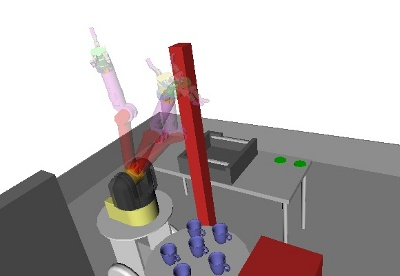
\includegraphics[width=10cm]{cppexample_ortrajectory.jpg}
\caption{Robot moving in random configurations.}
\end{DoxyImage}


Shows how to send a cubicaly interpolated trajectory to the robot controller. The actual trajectory consists of two points: the current configuration and the target configuration.


\begin{DoxyCode}
    TrajectoryBasePtr traj = RaveCreateTrajectory(penv,"");
    traj->Init(probot->GetActiveConfigurationSpecification());
    probot->GetActiveDOFValues(q); // get current values
    traj->Insert(0,q);
    q[0] = 0.5;
    traj->Insert(1,q);
    planningutils::RetimeActiveDOFTrajectory(probot,traj);
\end{DoxyCode}


The demo also adds a collision check at the target point to make sure robot is going to a collision free configuration.


\begin{DoxyCode}
    {
        RobotBase::RobotStateSaver saver(probot); // add a state saver so robot i
      s not moved permenantly
        probot->SetDOFValues(q);
        if( penv->CheckCollision(RobotBaseConstPtr(probot)) ) {
            continue; // robot in collision at final point, so reject
        }
    }
\end{DoxyCode}


In order for the path itself to be collision free, we would have to use planners.

{\bfseries Full Example Code:}


\begin{DoxyCodeInclude}

#include <openrave-core.h>
#include <vector>
#include <cstring>
#include <sstream>

#include <boost/thread/thread.hpp>
#include <boost/bind.hpp>
#include <openrave/planningutils.h>

using namespace OpenRAVE;
using namespace std;

#ifdef _WIN32
#define WIN32_LEAN_AND_MEAN
#include <windows.h>
#define usleep(micro) Sleep(micro/1000)
#endif

void SetViewer(EnvironmentBasePtr penv, const string& viewername)
{
    ViewerBasePtr viewer = RaveCreateViewer(penv,viewername);
    penv->AddViewer(viewer);
    viewer->main(true);
}

int main(int argc, char ** argv)
{
    string scenefilename = "data/lab1.env.xml";
    string viewername = "qtcoin";
    RaveInitialize(true);
    EnvironmentBasePtr penv = RaveCreateEnvironment();
    penv->SetDebugLevel(Level_Debug);

    boost::thread thviewer(boost::bind(SetViewer,penv,viewername)); // create the
       viewer
    usleep(300000); // wait for the viewer to init

    penv->Load(scenefilename);
    vector<RobotBasePtr> vrobots;
    penv->GetRobots(vrobots);
    RobotBasePtr probot = vrobots.at(0);
    std::vector<dReal> q;

    while(1) {
        {
            EnvironmentMutex::scoped_lock lock(penv->GetMutex()); // lock environ
      ment

            TrajectoryBasePtr traj = RaveCreateTrajectory(penv,"");
            traj->Init(probot->GetActiveConfigurationSpecification());
            probot->GetActiveDOFValues(q); // get current values
            traj->Insert(0,q);
            q[RaveRandomInt()%probot->GetDOF()] += RaveRandomFloat()-0.5; // move
       a random axis

            // check for collisions
            {
                RobotBase::RobotStateSaver saver(probot); // add a state saver so
       robot is not moved permenantly
                probot->SetDOFValues(q);
                if( penv->CheckCollision(RobotBaseConstPtr(probot)) ) {
                    continue; // robot in collision at final point, so reject
                }
            }

            traj->Insert(1,q);
            planningutils::RetimeActiveDOFTrajectory(traj,probot);
            probot->GetController()->SetPath(traj);
            // setting through the robot is also possible: probot->SetMotion(traj
      );
        }
        // unlock the environment and wait for the robot to finish
        while(!probot->GetController()->IsDone()) {
            usleep(1000);
        }
    }

    thviewer.join(); // wait for the viewer thread to exit
    penv->Destroy(); // destroy
    return 0;
}
\end{DoxyCodeInclude}
 